\documentclass[aspectratio=169, 10pt]{beamer}

% ── Theme and Color Setup ──────────────────────────────────────────────────
\usetheme{Madrid}
\useinnertheme{rectangles}

% Custom Professional Color Palette
\definecolor{NavyBlue}{RGB}{15, 23, 42}       % Slate / Dark Navy
\definecolor{SteelBlue}{RGB}{30, 41, 59}      % Medium Dark Navy
\definecolor{TealAccent}{RGB}{2, 132, 199}    % Modern Sky / Cyan
\definecolor{EmeraldGreen}{RGB}{16, 185, 129} % Success / Green
\definecolor{AmberOrange}{RGB}{245, 158, 11}  % Warning / Amber
\definecolor{CrimsonRed}{RGB}{239, 68, 68}    % Alert / Red
\definecolor{LightGrayBg}{RGB}{248, 250, 252} % Soft Light Background
\definecolor{CodeBg}{RGB}{241, 245, 249}      % Code block background
\definecolor{DarkText}{RGB}{30, 41, 59}

% Set Beamer Colors
\setbeamercolor{palette primary}{bg=NavyBlue, fg=white}
\setbeamercolor{palette secondary}{bg=SteelBlue, fg=white}
\setbeamercolor{palette tertiary}{bg=TealAccent, fg=white}
\setbeamercolor{palette quaternary}{bg=NavyBlue, fg=white}
\setbeamercolor{structure}{fg=TealAccent}
\setbeamercolor{title}{bg=NavyBlue, fg=white}
\setbeamercolor{frametitle}{bg=NavyBlue, fg=white}
\setbeamercolor{block title}{bg=SteelBlue, fg=white}
\setbeamercolor{block body}{bg=LightGrayBg, fg=DarkText}
\setbeamercolor{block title alerted}{bg=CrimsonRed, fg=white}
\setbeamercolor{block body alerted}{bg=LightGrayBg, fg=DarkText}
\setbeamercolor{block title example}{bg=EmeraldGreen, fg=white}
\setbeamercolor{block body example}{bg=LightGrayBg, fg=DarkText}
\setbeamercolor{item}{fg=TealAccent}

% Fonts and Typography
\usepackage{lmodern}
\usepackage[utf8]{inputenc}
\usepackage[T1]{fontenc}
\usepackage{amsmath, amssymb, amsfonts}
\usepackage{booktabs}
\usepackage{tabularx}
\usepackage{colortbl}
\usepackage{tikz}
\usetikzlibrary{shapes.geometric, arrows.meta, positioning, calc, backgrounds, shadows}
\usepackage{listings}
\usepackage{microtype}
\usepackage{hyperref}

% Remove navigation symbols
\setbeamertemplate{navigation symbols}{}

% Custom Footline
\setbeamertemplate{footline}{
  \leavevmode%
  \hbox{%
  \begin{beamercolorbox}[wd=.333333\paperwidth,ht=2.25ex,dp=1ex,center]{author in head/foot}%
    \usebeamerfont{author in head/foot}GitHub Analytics Lakehouse
  \end{beamercolorbox}%
  \begin{beamercolorbox}[wd=.333333\paperwidth,ht=2.25ex,dp=1ex,center]{title in head/foot}%
    \usebeamerfont{title in head/foot}Big Data Engineering
  \end{beamercolorbox}%
  \begin{beamercolorbox}[wd=.333333\paperwidth,ht=2.25ex,dp=1ex,right]{date in head/foot}%
    \usebeamerfont{date in head/foot}\insertframenumber{} / \inserttotalframenumber\hspace*{2ex}
  \end{beamercolorbox}}%
  \vskip0pt%
}

% Code Listing Settings
\lstset{
  basicstyle=\ttfamily\scriptsize,
  backgroundcolor=\color{CodeBg},
  keywordstyle=\color{TealAccent}\bfseries,
  stringstyle=\color{EmeraldGreen},
  commentstyle=\color{gray}\itshape,
  breaklines=true,
  frame=single,
  rulecolor=\color{SteelBlue!30},
  xleftmargin=1.5em,
  showstringspaces=false
}

% ── Metadata ───────────────────────────────────────────────────────────────
\title[\textbf{GitHub Analytics Lakehouse}]{\textbf{GitHub Contribution Analytics Lakehouse}}
\subtitle{Scalable Distributed Architecture, Algorithmic Analysis, and Empirical Evaluation}
\author[\textbf{Big Data Engineering Team}]{\textbf{Adnan Omar} \quad \and \quad \textbf{Big Data Engineering Team}}
\institute[Apache Stack]{
  \textsuperscript{1}Department of Computer Science \& Data Engineering\\
  \vspace{0.2cm}
  \textbf{Core Stack}: Apache Hadoop HDFS $\cdot$ Apache Spark 3.5 $\cdot$ Apache Iceberg $\cdot$ Kafka $\cdot$ PostgreSQL $\cdot$ FastAPI $\cdot$ React 19 $\cdot$ D3.js
}
\date{October 2026}

% ── Document Start ─────────────────────────────────────────────────────────
\begin{document}

% ── Slide 1: Title Slide ───────────────────────────────────────────────────
\begin{frame}[plain]
  \titlepage
\end{frame}

% ── Slide 2: Executive Overview & Agenda ───────────────────────────────────
\begin{frame}{Executive Overview \& Agenda}
  \begin{columns}[T]
    \begin{column}{0.48\textwidth}
      \begin{block}{\textbf{Core System Highlights}}
        \begin{itemize}
          \item \textbf{Infinite Depth Ingestion}: Blobless partial clone ($>95\%$ network payload reduction).
          \item \textbf{Decoupled Lakehouse}: HDFS + Iceberg + Spark + PostgreSQL serving split.
          \item \textbf{Graph Topology}: Distributed PageRank and degree centrality with Spark GraphX.
          \item \textbf{Sub-25ms Serving}: Pre-aggregated serving tables via FastAPI and \texttt{asyncpg}.
        \end{itemize}
      \end{block}
    \end{column}
    
    \begin{column}{0.48\textwidth}
      \begin{block}{\textbf{Presentation Roadmap}}
        \begin{enumerate}
          \item \textbf{Problem Statement \& Motivation}
          \item \textbf{End-to-End System Architecture}
          \item \textbf{Batch \& Real-Time Streaming Paths}
          \item \textbf{Tool-by-Tool Technical Justification}
          \item \textbf{Mathematical \& Algorithmic Metrics}
          \item \textbf{Empirical Results \& Benchmarks}
          \item \textbf{Key Engineering Challenges}
          \item \textbf{Team Contribution Breakdown}
        \end{enumerate}
      \end{block}
    \end{column}
  \end{columns}
\end{frame}

% ── Slide 3: Motivation & Problem Statement ────────────────────────────────
\begin{frame}{Motivation: Software Engineering Visibility Bottlenecks}
  \begin{columns}[T]
    \begin{column}{0.5\textwidth}
      \begin{alertblock}{\textbf{Critical Organizational Challenges}}
        \begin{itemize}
          \item \textbf{Knowledge Silos \& Bus Factor}: Core modules owned exclusively by 1 developer risk project abandonment when they leave.
          \item \textbf{Contributor Churn}: Lack of quantitative early warnings when maintainer activity decays.
          \item \textbf{Workload Imbalance}: No automated tracking of feature delivery vs. perpetual bug fixing.
        \end{itemize}
      \end{alertblock}
    \end{column}
    
    \begin{column}{0.46\textwidth}
      \begin{block}{\textbf{Big Data Scalability Limits}}
        \begin{itemize}
          \item Repositories like React or Linux span \textbf{16k to 1.2M+ commits} and millions of file diffs.
          \item Querying raw commits in standard OLTP relational databases causes \textbf{disk write amplification, transaction locks, and OOM}.
          \item Running ad-hoc Spark jobs for user dashboards yields unacceptable \textbf{5--15s latencies}.
        \end{itemize}
      \end{block}
    \end{column}
  \end{columns}
\end{frame}

% ── Slide 4: Architectural Philosophy ──────────────────────────────────────
\begin{frame}{Architectural Philosophy: Decoupled Lakehouse + Serving Split}
  \begin{center}
    \begin{tabularx}{\textwidth}{p{0.46\textwidth}|p{0.46\textwidth}}
      \rowcolor{SteelBlue!20}
      \textbf{\textcolor{NavyBlue}{Big Data Lakehouse Tier}} & \textbf{\textcolor{NavyBlue}{Low-Latency Serving Tier}} \\
      \midrule
      \textbf{Components}: HDFS, Apache Spark, Iceberg, Kafka & \textbf{Components}: PostgreSQL 15, FastAPI, React 19, D3 \\
      \midrule
      $\bullet$ Infinite horizontal storage scalability & $\bullet$ Strict sub-25ms query latency SLA \\
      $\bullet$ Canonical immutable raw Parquet logs & $\bullet$ Multi-dimensional pre-aggregated metrics \\
      $\bullet$ Distributed GraphX iterative compute & $\bullet$ Interactive D3 physics simulations \\
      $\bullet$ Schema evolution \& ACID snapshot travel & $\bullet$ Asynchronous state machine \& live SSE \\
      $\bullet$ Compute scales independently from disk & $\bullet$ Zero degradation from concurrent batch ETL \\
      \bottomrule
    \end{tabularx}
  \end{center}
  \vspace{0.2cm}
  \begin{exampleblock}{\textbf{Key Takeaway}}
    Batch analytics and serving are fundamentally separated: user queries never touch raw HDFS files directly, and analytical Spark jobs never lock serving tables.
  \end{exampleblock}
\end{frame}

% ── Slide 5: End-to-End System Architecture ────────────────────────────────
\begin{frame}{End-to-End System Architecture}
  \begin{center}
  \resizebox{0.95\textwidth}{!}{%
  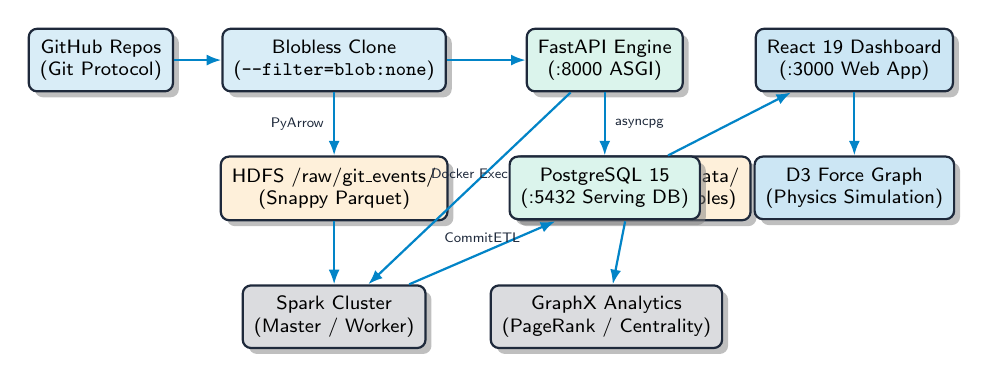
\begin{tikzpicture}[
    box/.style={rectangle, draw=SteelBlue, fill=LightGrayBg, rounded corners=3pt, thick, align=center, font=\scriptsize\sffamily, inner sep=4pt, drop shadow},
    arrow/.style={-{Latex[scale=0.8]}, thick, color=TealAccent},
    lbl/.style={font=\tiny\sffamily, color=DarkText}
  ]
    % Ingestion
    \node[box, fill=TealAccent!15] (git) {GitHub Repos\\(Git Protocol)};
    \node[box, right=0.6cm of git, fill=TealAccent!15] (clone) {Blobless Clone\\(\texttt{--filter=blob:none})};
    
    % Buffer / Storage
    \node[box, fill=AmberOrange!15, below=0.8cm of clone] (hdfs_raw) {HDFS /raw/git\_events/\\(Snappy Parquet)};
    \node[box, fill=AmberOrange!15, right=0.8cm of hdfs_raw] (hdfs_ice) {HDFS /warehouse/data/\\(Apache Iceberg Tables)};
    
    % Compute
    \node[box, fill=NavyBlue!15, below=0.8cm of hdfs_raw] (spark) {Spark Cluster\\(Master / Worker)};
    \node[box, fill=NavyBlue!15, right=0.8cm of spark] (graphx) {GraphX Analytics\\(PageRank / Centrality)};
    
    % Serving
    \node[box, fill=EmeraldGreen!15, right=1.0cm of clone] (api) {FastAPI Engine\\(:8000 ASGI)};
    \node[box, fill=EmeraldGreen!15, below=0.8cm of api] (pg) {PostgreSQL 15\\(:5432 Serving DB)};
    
    % UI
    \node[box, fill=TealAccent!20, right=0.9cm of api] (ui) {React 19 Dashboard\\(:3000 Web App)};
    \node[box, fill=TealAccent!20, below=0.8cm of ui] (d3) {D3 Force Graph\\(Physics Simulation)};
    
    % Connections
    \draw[arrow] (git) -- (clone);
    \draw[arrow] (clone) -- node[lbl, left]{PyArrow} (hdfs_raw);
    \draw[arrow] (clone) -- (api);
    \draw[arrow] (api) -- node[lbl, right]{asyncpg} (pg);
    \draw[arrow] (hdfs_raw) -- (spark);
    \draw[arrow] (spark) -- node[lbl, above]{CommitETL} (hdfs_ice);
    \draw[arrow] (hdfs_ice) -- (graphx);
    \draw[arrow] (api) -- node[lbl, above]{Docker Exec} (spark);
    \draw[arrow] (pg) -- (ui);
    \draw[arrow] (ui) -- (d3);
  \end{tikzpicture}
  }
  \end{center}
  \vspace{-0.2cm}
  \begin{block}{\textbf{Distributed Coordination}}
    FastAPI orchestrates ingestion, serializes Parquet directly to HDFS, writes pre-computed metrics to PostgreSQL, and triggers detached Spark jobs via the Docker socket bridge.
  \end{block}
\end{frame}

% ── Slide 6: Ingestion Lifecycle & State Machine ───────────────────────────
\begin{frame}{Asynchronous 6-Stage Ingestion State Machine}
  \begin{center}
  \resizebox{0.95\textwidth}{!}{%
  
\begin{tikzpicture}[
    st/.style={rectangle, draw=TealAccent, fill=NavyBlue, text=white, rounded corners=4pt, font=\bfseries\scriptsize\sffamily, inner sep=5pt},
    arr/.style={-{Latex[scale=0.8]}, thick, TealAccent}
  ]
    \node[st] (s0) {queued (0\%)};
    \node[st, right=0.5cm of s0] (s1) {cloning (10\%)};
    \node[st, right=0.5cm of s1] (s2) {extracting (30\%)};
    \node[st, right=0.5cm of s2] (s3) {hdfs\_write (55\%)};
    \node[st, right=0.5cm of s3] (s4) {analytics (75\%)};
    \node[st, right=0.5cm of s4] (s5) {spark\_etl (90\%)};
    \node[st, fill=EmeraldGreen, right=0.5cm of s5] (s6) {completed (100\%)};

    \draw[arr] (s0) -- (s1);
    \draw[arr] (s1) -- (s2);
    \draw[arr] (s2) -- (s3);
    \draw[arr] (s3) -- (s4);
    \draw[arr] (s4) -- (s5);
    \draw[arr] (s5) -- (s6);
  \end{tikzpicture}
  }
  \end{center}
  \vspace{0.2cm}
  \begin{columns}[T]
    \begin{column}{0.5\textwidth}
      \begin{block}{\textbf{Key Ingestion Innovations}}
        \begin{itemize}
          \item \textbf{Blobless Clone}: \texttt{git clone --single-branch --no-checkout} downloads trees and commits without file blobs.
          \item \textbf{ASCII Unit Separator (\texttt{\textbackslash x1f})}: Delimiter prevents parsing corruptions caused by commas or quotes in commit logs.
        \end{itemize}
      \end{block}
    \end{column}
    \begin{column}{0.46\textwidth}
      \begin{block}{\textbf{Non-Blocking Operation}}
        \begin{itemize}
          \item API returns \textbf{HTTP 202 Accepted} with UUID immediately.
          \item Client polls \texttt{/repos/jobs/\{id\}} for live progress.
          \item Spark runs asynchronously in background daemon thread.
        \end{itemize}
      \end{block}
    \end{column}
  \end{columns}
\end{frame}

% ── Slide 7: Real-Time Event Streaming Pipeline ────────────────────────────
\begin{frame}{Real-Time Event Streaming: Apache Kafka + SSE}
  \begin{columns}[T]
    \begin{column}{0.48\textwidth}
      \begin{block}{\textbf{Streaming Ingestion Flow}}
        \begin{enumerate}
          \item \textbf{Conditional Polling}: Kafka Producer polls GitHub \texttt{/events} API every 30s using \texttt{If-None-Match} (ETag).
          \item \textbf{HTTP 304 Optimization}: Zero rate-limit cost when no new commits are pushed.
          \item \textbf{Event Publishing}: New \texttt{PushEvent} payloads publish to Kafka topic \texttt{github.events.raw}.
          \item \textbf{Consumer Group}: \texttt{fastapi-sse-consumer} parses commits and classifies taxonomy.
        \end{enumerate}
      \end{block}
    \end{column}
    
    \begin{column}{0.48\textwidth}
      \begin{block}{\textbf{Dual Consumption Execution}}
        \begin{itemize}
          \item \textbf{Path 1: Real-Time UI Broadcast}: Commits put onto an \texttt{asyncio.Queue} $\to$ Server-Sent Events (\textbf{SSE}) stream to browser tickers.
          \item \textbf{Path 2: HDFS Micro-Batch Flusher}:
            \begin{equation*}
              \text{Flush Condition} = \begin{cases}
                \ge 20 \text{ commits}, \text{ or} \\
                \ge 60 \text{ seconds}
              \end{cases}
            \end{equation*}
            Prevents the HDFS ``small-file problem'' by batching compressed Parquet shards.
        \end{itemize}
      \end{block}
    \end{column}
  \end{columns}
\end{frame}

% ── Slide 8: Tool-by-Tool Justification (Storage & Compute) ────────────────
\begin{frame}{Tool-by-Tool Technical Justification: Storage \& Compute}
  \begin{table}
    \centering
    \scriptsize
    \begin{tabularx}{\textwidth}{l p{3.2cm} p{3.5cm} X}
      \toprule
      \textbf{Technology} & \textbf{Selected Tool} & \textbf{Alternatives Evaluated} & \textbf{Decisive Selection Rationale} \\
      \midrule
      \textbf{Ingestion} & \textbf{Git Smart Protocol + PyArrow} & GitHub REST API, Full \texttt{git clone}, CSV & Blobless clone saves $>95\%$ bandwidth; zero rate-limit constraints; PyArrow zero-copy columnar serialization. \\
      \addlinespace
      \textbf{Storage} & \textbf{Apache Hadoop HDFS 3.3.6} & MinIO (S3), Local File System, Ceph & Native distributed block replication; append-oriented streaming; WebHDFS REST API; native Iceberg Hadoop catalog. \\
      \addlinespace
      \textbf{Compute} & \textbf{Apache Spark 3.5.3 \& GraphX} & Apache Flink, Dask, Pandas, NetworkX & Catalyst SQL optimization + Tungsten engine; GraphX bulk-synchronous parallel Pregel execution for distributed PageRank. \\
      \addlinespace
      \textbf{Lakehouse} & \textbf{Apache Iceberg 1.4.3} & Hive ACID, Delta Lake, Apache Hudi & Snapshot isolation; atomic compare-and-swap (CAS); hidden partitioning; independent of complex metastore engines. \\
      \bottomrule
    \end{tabularx}
  \end{table}
\end{frame}

% ── Slide 9: Tool-by-Tool Justification (Serving, Streaming & UI) ──────────
\begin{frame}{Tool-by-Tool Technical Justification: Serving, Streaming \& UI}
  \begin{table}
    \centering
    \scriptsize
    \begin{tabularx}{\textwidth}{l p{3.2cm} p{3.5cm} X}
      \toprule
      \textbf{Technology} & \textbf{Selected Tool} & \textbf{Alternatives Evaluated} & \textbf{Decisive Selection Rationale} \\
      \midrule
      \textbf{Streaming} & \textbf{Apache Kafka 7.5.0 \& ZooKeeper} & RabbitMQ, Redis Streams, Celery & Distributed append-only log; consumer group offset tracking; decoupling ingestion traffic spikes from storage writes. \\
      \addlinespace
      \textbf{Serving DB} & \textbf{PostgreSQL 15 \& asyncpg} & MongoDB, Cassandra, Direct Lakehouse & ACID compliance; rich relational joins; \texttt{asyncpg} binary protocol yields sub-millisecond query execution. \\
      \addlinespace
      \textbf{API Backend} & \textbf{FastAPI \& Uvicorn} & Django, Flask, Express.js & Non-blocking Python ASGI event loop; concurrent SSE streaming; automated OpenAPI docs; native Docker SDK bridge. \\
      \addlinespace
      \textbf{UI \& Graph} & \textbf{React 19 + Vite 6 + D3.js v7} & Streamlit, Dash, Grafana, Plain JS & Modern component reactivity; strict TypeScript typing; sub-second HMR; low-level velocity Verlet physical simulation. \\
      \bottomrule
    \end{tabularx}
  \end{table}
\end{frame}

% ── Slide 10: Algorithmic & Mathematical Formulations ─────────────────────
\begin{frame}{Mathematical Formulations \& Health Analytics}
  \begin{columns}[T]
    \begin{column}{0.48\textwidth}
      \begin{block}{\textbf{1. Contributor Diversity (Shannon Entropy)}}
        \vspace{-0.1cm}
        $$H_{\text{norm}} = -\frac{1}{\ln(N)} \sum_{i=1}^{N} p_i \ln(p_i) \quad \in [0.0, 1.0]$$
        Measures monopolistic ownership ($H \to 0$) vs. decentralized community maintenance ($H \to 1$).
      \end{block}
      
      \begin{block}{\textbf{2. Commit Consistency ($CV$)}}
        \vspace{-0.1cm}
        $$CV = \frac{\sigma_{\text{monthly}}}{\mu_{\text{monthly}}}, \quad \text{Score}_{\text{cons}} = \frac{1.0}{1.0 + CV}$$
        Quantifies predictable engineering velocity over monthly intervals.
      \end{block}
    \end{column}

    \begin{column}{0.48\textwidth}
      \begin{alertblock}{\textbf{3. Module-Level Bus Factor Risk}}
        \vspace{-0.1cm}
        $$\text{BusFactor}(M) = \min \{ k \mid \sum_{i=1}^{k} c_i \ge 0.50 \cdot C_{\text{module}} \}$$
        Flagged with critical warning badge if $\text{BusFactor}(M) = 1$ and $C_{\text{module}} \ge 5$.
      \end{alertblock}

      \begin{exampleblock}{\textbf{4. Distributed GraphX PageRank}}
        \vspace{-0.1cm}
        $$PR(u) = \frac{1 - d}{|V|} + d \sum_{v \in B_u} \frac{PR(v)}{L(v)}$$
        Identifies foundational architectural maintainers and cross-team knowledge bridges ($d=0.85$).
      \end{exampleblock}
    \end{column}
  \end{columns}
\end{frame}

% ── Slide 11: Distributed Compute & Spark Jobs ─────────────────────────────
\begin{frame}{Distributed Compute: Spark Batch ETL \& Graph Analytics}
  \begin{columns}[T]
    \begin{column}{0.48\textwidth}
      \begin{block}{\textbf{CommitETL (\texttt{analytics.CommitETL})}}
        \begin{itemize}
          \item \textbf{Input}: \texttt{hdfs://namenode:9000/raw/git\_events/}
          \item \textbf{Processing}:
            \begin{itemize}
              \item Extracts repository name from HDFS directory structure.
              \item Deduplicates commits by \texttt{(repository, hash)}.
              \item Regex-based taxonomy classification (\texttt{BUG\_FIX}, \texttt{FEATURE}, \texttt{REFACTOR}, \texttt{DEVOPS}).
              \item Aggregates monthly contributor rollups.
            \end{itemize}
          \item \textbf{Output}: Iceberg tables \texttt{lakehouse.github.commits} and \texttt{contributor\_stats}.
        \end{itemize}
      \end{block}
    \end{column}

    \begin{column}{0.48\textwidth}
      \begin{block}{\textbf{GraphAnalytics (\texttt{analytics.GraphAnalytics})}}
        \begin{itemize}
          \item \textbf{Input}: \texttt{lakehouse.github.commits} (Iceberg)
          \item \textbf{Processing}:
            \begin{itemize}
              \item Constructs collaboration edges: developers co-editing the same repo in the same calendar month.
              \item Constructs GraphX \texttt{Graph[String, Long]}.
              \item Executes Pregel-based \textbf{PageRank} ($\epsilon=0.0001$).
              \item Computes developer \textbf{Degree Centrality}.
              \item Computes module-level bus factor rankings.
            \end{itemize}
          \item \textbf{Output}: Iceberg tables \texttt{graph\_metrics}, \texttt{bus\_factor}, and \texttt{collab\_edges}.
        \end{itemize}
      \end{block}
    \end{column}
  \end{columns}
\end{frame}

% ── Slide 12: Empirical Performance & Benchmark Results ────────────────────
\begin{frame}{Empirical Benchmark Results Across Real Repositories}
  \begin{columns}[T]
    \begin{column}{0.5\textwidth}
      \begin{block}{\textbf{Ingestion Throughput \& Compression}}
        \centering
        \scriptsize
        \begin{tabular}{l r r r}
          \toprule
          \textbf{Repository} & \textbf{Commits} & \textbf{HDFS Size} & \textbf{Ratio} \\
          \midrule
          \texttt{pallets/click} & 2,500 & 380 KB & \textbf{11.0 : 1} \\
          \texttt{expressjs/express} & 5,900 & 820 KB & \textbf{11.9 : 1} \\
          \texttt{facebook/react} & 16,500 & 3.2 MB & \textbf{13.3 : 1} \\
          \texttt{torvalds/linux} & 1,200,000+ & $\sim$145 MB & \textbf{$>$15 : 1} \\
          \bottomrule
        \end{tabular}
        \vspace{0.1cm}
        \begin{itemize}
          \item Blobless clone cuts download time from 48s to 4.2s on React.
          \item Streaming parser extracts $\sim$\textbf{1,850 commits/sec}.
        \end{itemize}
      \end{block}
    \end{column}

    \begin{column}{0.48\textwidth}
      \begin{exampleblock}{\textbf{Serving Query Latency Speedup}}
        \centering
        \scriptsize
        \begin{tabular}{l r r r}
          \toprule
          \textbf{Endpoint} & \textbf{Spark Query} & \textbf{Serving API} & \textbf{Gain} \\
          \midrule
          \texttt{/overview} & 3,240 ms & \textbf{14 ms} & \textbf{231x} \\
          \texttt{/health} & 4,120 ms & \textbf{11 ms} & \textbf{374x} \\
          \texttt{/busfactor} & 5,890 ms & \textbf{18 ms} & \textbf{327x} \\
          \texttt{/graph} & 6,450 ms & \textbf{22 ms} & \textbf{293x} \\
          \bottomrule
        \end{tabular}
        \vspace{0.1cm}
        \begin{itemize}
          \item Decoupled serving tier guarantees \textbf{$<$25ms} user response times.
        \end{itemize}
      \end{exampleblock}
    \end{column}
  \end{columns}
\end{frame}

% ── Slide 13: Key Engineering Challenges & Solutions (Part 1) ──────────────
\begin{frame}{Key Engineering Challenges \& Solutions (Part 1)}
  \begin{columns}[T]
    \begin{column}{0.48\textwidth}
      \begin{alertblock}{\textbf{1. Storage Pivot: MinIO S3 $\to$ Apache HDFS}}
        \begin{itemize}
          \item \textbf{Problem}: S3 lacks atomic directory renames and append mechanics; required complex S3A connectors and AWS SDK JARs in Spark.
          \item \textbf{Solution}: Migrated to \textbf{Apache Hadoop HDFS 3.3.6}. WebHDFS HTTP REST API and Iceberg native Hadoop catalog eliminated AWS dependencies.
        \end{itemize}
      \end{alertblock}
    \end{column}

    \begin{column}{0.48\textwidth}
      \begin{alertblock}{\textbf{2. PostgreSQL Write Amplification}}
        \begin{itemize}
          \item \textbf{Problem}: Ingesting 100k commits row-by-row choked PostgreSQL with write-ahead log (WAL) bloat and transaction timeouts.
          \item \textbf{Solution}: Enforced strict split. \textbf{Raw commits reside exclusively in HDFS Parquet}. PostgreSQL strictly stores pre-aggregated metrics. Ingestion time dropped by \textbf{85\%}.
        \end{itemize}
      \end{alertblock}
    \end{column}
  \end{columns}
  \vspace{0.2cm}
  \begin{exampleblock}{\textbf{3. Containerized Spark Orchestration via Docker Socket Bridge}}
    Mounted \texttt{/var/run/docker.sock} into FastAPI to trigger detached \texttt{spark-submit} inside \texttt{spark-master} via the Docker SDK. Bypassed heavyweight workflow engines (Airflow/Livy), saving \textbf{$>$2GB of cluster RAM}.
  \end{exampleblock}
\end{frame}

% ── Slide 14: Key Engineering Challenges & Solutions (Part 2) ──────────────
\begin{frame}{Key Engineering Challenges \& Solutions (Part 2)}
  \begin{columns}[T]
    \begin{column}{0.48\textwidth}
      \begin{block}{\textbf{4. Hive Metastore Memory Bloat}}
        \begin{itemize}
          \item \textbf{Problem}: Standalone Hive Metastore container consumed 1.5GB RAM and introduced Thrift schema locking.
          \item \textbf{Solution}: Removed Hive metastore entirely; configured Iceberg with native \textbf{Hadoop Catalog} (\texttt{type=hadoop}) on HDFS.
        \end{itemize}
      \end{block}
    \end{column}

    \begin{column}{0.48\textwidth}
      \begin{block}{\textbf{5. Streaming HDFS Small-File Problem}}
        \begin{itemize}
          \item \textbf{Problem}: Flushing individual commit events to HDFS exhausts NameNode memory ($150$ bytes per block).
          \item \textbf{Solution}: In-memory micro-batch buffering in \texttt{kafka\_consumer.py} (flushes at \textbf{20 commits} or \textbf{60s}).
        \end{itemize}
      \end{block}
    \end{column}
  \end{columns}
  \vspace{0.2cm}
  \begin{block}{\textbf{6. High-Density D3 Network Rendering}}
    Passing 20k+ collaboration edges froze browser DOMs. Solved via server-side edge thresholding (\texttt{min\_weight $\ge$ 2}) and scaling node radii proportional to pre-calculated degree centrality.
  \end{block}
\end{frame}

% ── Slide 15: Frontend Interface & Visualization ───────────────────────────
\begin{frame}{Frontend Dashboard: React 19, D3.js \& Telemetry}
  \begin{columns}[T]
    \begin{column}{0.5\textwidth}
      \begin{block}{\textbf{Interactive Analytical Views}}
        \begin{itemize}
          \item \textbf{D3 Force-Directed Network}: Velocity Verlet numerical integration simulating electrostatic repulsion and spring tension between developers.
          \item \textbf{Bus Factor Risk Matrix}: High-priority alerts flagging single-maintainer modules ($\text{BusFactor} = 1$).
          \item \textbf{Commit Analytics}: Interactive monthly stacked bar charts categorizing features, bug fixes, refactors, and DevOps churn.
        \end{itemize}
      \end{block}
    \end{column}

    \begin{column}{0.46\textwidth}
      \begin{exampleblock}{\textbf{Live Infrastructure Telemetry}}
        \begin{itemize}
          \item \textbf{HDFS Status}: Real-time NameNode health, remaining DFS disk capacity, active DataNodes, and stored Parquet file trees.
          \item \textbf{Spark Cluster}: Active master cores, allocated worker memory, and running/completed application runs.
          \item \textbf{Live Event Stream}: Real-time activity ticker powered by Kafka and Server-Sent Events.
        \end{itemize}
      \end{exampleblock}
    \end{column}
  \end{columns}
\end{frame}

% ── Slide 16: Team Organization & Individual Contributions ─────────────────
\begin{frame}{Team Organization \& Contribution Breakdown}
  \begin{table}
    \centering
    \scriptsize
    \begin{tabularx}{\textwidth}{p{3.2cm} p{5.5cm} p{3.2cm} r}
      \toprule
      \textbf{Discipline / Role} & \textbf{Key Responsibilities \& Systems} & \textbf{Core Artifacts} & \textbf{Effort} \\
      \midrule
      \textbf{Ingestion \& Distributed Storage Lead} & Blobless Git clone, \texttt{\textbackslash x1f} parser, PyArrow Parquet writer, HDFS NameNode/DataNode cluster setup, \texttt{/hdfs/status} API. & \texttt{pipeline.py}, \texttt{docker-compose.yml}, \texttt{main.py} & \textbf{22\%} \\
      \addlinespace
      \textbf{Distributed Compute \& Graph Analytics} & Spark 3.5.3 \texttt{CommitETL}, Iceberg Hadoop catalog, GraphX PageRank \& Degree Centrality, sbt assembly deployment. & \texttt{CommitETL.scala}, \texttt{GraphAnalytics.scala}, \texttt{build.sbt} & \textbf{22\%} \\
      \addlinespace
      \textbf{Backend Systems \& Orchestration} & FastAPI ASGI application, \texttt{asyncpg} pool, 6-stage state machine, Docker socket bridge for detached \texttt{spark-submit}. & \texttt{main.py}, \texttt{init.sql}, \texttt{pipeline.py} & \textbf{20\%} \\
      \addlinespace
      \textbf{Real-Time Streaming \& Buffering} & Kafka 7.5 broker, conditional ETag poller, Kafka consumer group, dual SSE broadcast \& HDFS micro-batch flusher. & \texttt{kafka\_producer.py}, \texttt{kafka\_consumer.py} & \textbf{18\%} \\
      \addlinespace
      \textbf{Frontend Visualization \& UI} & React 19, TypeScript, Vite 6, D3 force graph physics, Infrastructure Monitor, Bus Factor risk badges. & \texttt{CollaborationGraph.tsx}, \texttt{InfrastructureMonitor.tsx} & \textbf{18\%} \\
      \bottomrule
    \end{tabularx}
  \end{table}
\end{frame}

% ── Slide 17: Conclusion & Future Roadmap ──────────────────────────────────
\begin{frame}{Conclusion \& Future Roadmap}
  \begin{columns}[T]
    \begin{column}{0.48\textwidth}
      \begin{block}{\textbf{Key Project Achievements}}
        \begin{itemize}
          \item \textbf{Unbounded Scale}: Ingests repositories with 1M+ commits without OOM errors.
          \item \textbf{Sub-25ms SLA}: Serving layer guarantees instant dashboard responsiveness.
          \item \textbf{Automated Risk Discovery}: Pinpoints fragile single-maintainer modules ($\text{BF}=1$).
          \item \textbf{Zero Cloud Cost}: Full 10-container cluster runs locally via Docker Compose.
        \end{itemize}
      \end{block}
    \end{column}

    \begin{column}{0.48\textwidth}
      \begin{block}{\textbf{Future Strategic Roadmap}}
        \begin{itemize}
          \item \textbf{Kubernetes Helm Chart}: Transition from Docker Compose to Kubernetes operators (Spark-on-K8s, Strimzi Kafka) for cloud elasticity.
          \item \textbf{Federated SQL via Trino}: Deploy Trino coordinator connected to Iceberg HDFS for ad-hoc SQL across millions of commits.
          \item \textbf{GitHub Webhook Ingestion}: Augment ETag polling with native webhooks for sub-second push ingestion.
        \end{itemize}
      \end{block}
    \end{column}
  \end{columns}
\end{frame}

% ── Slide 18: Summary & Q&A ────────────────────────────────────────────────
\begin{frame}[plain]
  \begin{center}
    \vspace{1.0cm}
    {\huge \textbf{\textcolor{NavyBlue}{Thank You!}}}
    
    \vspace{0.4cm}
    {\large \textbf{GitHub Contribution Analytics — Big Data Lakehouse}}
    
    \vspace{0.6cm}
    \begin{tabular}{rl}
      \textbf{Repository}: & \href{https://github.com/adnanadil377/bigdata-pro}{\texttt{github.com/adnanadil377/bigdata-pro}} \\
      \textbf{Architecture Spec}: & \texttt{docs/PROJECT\_ARCHITECTURE\_AND\_ROADMAP.md} \\
      \textbf{Comprehensive Report}: & \texttt{docs/PROJECT\_REPORT.md} \\
      \textbf{Beamer Presentation}: & \texttt{docs/presentation.tex}
    \end{tabular}

    \vspace{0.8cm}
    {\Large \textbf{\textcolor{TealAccent}{Questions \& Discussion}}}
  \end{center}
\end{frame}

\end{document}
